\documentclass[conference]{IEEEtran}
\usepackage{amsmath,booktabs,url}
\usepackage{tikz}
\usetikzlibrary{positioning,arrows.meta}
\title{DietSense: A Conversational Domain AI Agent for Daily Calorie Intake Analysis}
\author{\IEEEauthorblockN{Author Name}\IEEEauthorblockA{National Taiwan Ocean University\\Taiwan}}
\begin{document}
\maketitle
\begin{abstract}
Manual dietary logging requires users to identify foods, estimate portions, and locate nutritional information. This work proposes DietSense, a conversational agent designed to support daily dietary self-monitoring, particularly for Taiwanese meals. The proposed architecture separates language understanding, evidence retrieval, deterministic nutrient calculation, and user-confirmed logging. A bounded clarification loop handles missing portions and uncertain food matches. Model Context Protocol (MCP) is considered as an interface for future tool integration, while OpenSpec documents requirements and acceptance scenarios. The current repository contains a deterministic calculation scaffold and synthetic demonstration records; live retrieval and conversational orchestration remain planned. An evaluation protocol is presented for estimating accuracy, usability, and evidence completeness without claiming unmeasured performance.
\end{abstract}
\begin{IEEEkeywords}
Conversational agents, nutrition informatics, retrieval, dietary logging, MCP, OpenSpec.
\end{IEEEkeywords}
\section{Introduction}
Dietary self-monitoring involves recording food identity, preparation, and quantity. A conversational interface may reduce the effort required to enter these attributes, but natural language often leaves essential details unspecified. For example, a bowl of beef noodles may contain different quantities of noodles, meat, broth, and oil. A plausible language-model response is not necessarily a reliable nutritional estimate.

DietSense addresses this challenge by proposing a modular system that grounds calculations in identifiable food records and separates numerical operations from language generation. The design targets Mandarin and English descriptions with particular attention to Taiwanese dishes. The project is intended for educational wellness self-monitoring, not clinical diagnosis or treatment.

The contributions of this draft are a modular architecture, an explicit evidence and uncertainty workflow, and a prospective evaluation protocol. The implementation status is distinguished from the proposed functionality throughout.
\section{Background and Related Work}
FoodData Central provides a public source of food composition information \cite{usda}. Taiwan's food composition resources provide a complementary starting point for local dishes \cite{taiwan}. Differences in cooking methods and serving sizes require careful matching rather than direct substitution between records.

Retrieval-augmented generation (RAG) combines language generation with retrieved information \cite{rag}. Tool-oriented reasoning approaches such as ReAct motivate the separation between reasoning and external actions \cite{react}. DietSense adopts these concepts at the design level; an LLM-driven retrieval loop has not yet been implemented. MCP offers a standardized interface between AI applications and external tools \cite{mcp}. OpenSpec provides a specification-driven workflow for defining changes and acceptance scenarios \cite{openspec}.
\section{System Architecture}
Figure~\ref{fig:arch} summarizes the proposed pipeline. The planner identifies intent and selects retrieval or calculation operations. The retrieval stage returns candidate records with source identifiers, preparation descriptions, and nutrient units. The analytics engine computes quantities explicitly, and the output module reports assumptions and requests confirmation before logging.
\begin{figure}[!t]
\centering
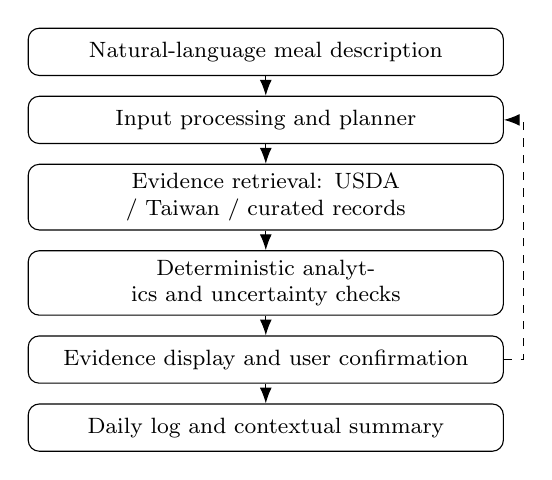
\begin{tikzpicture}[node distance=2.5mm, every node/.style={font=\footnotesize}, b/.style={draw,rounded corners,align=center,text width=5.8cm,minimum height=6mm},a/.style={-{Latex[length=2mm]}}]
\node[b] (u) {Natural-language meal description};
\node[b,below=of u] (p) {Input processing and planner};
\node[b,below=of p] (r) {Evidence retrieval: USDA / Taiwan / curated records};
\node[b,below=of r] (c) {Deterministic analytics and uncertainty checks};
\node[b,below=of c] (o) {Evidence display and user confirmation};
\node[b,below=of o] (d) {Daily log and contextual summary};
\draw[a] (u)--(p);\draw[a](p)--(r);\draw[a](r)--(c);\draw[a](c)--(o);\draw[a](o)--(d);
\draw[a,dashed] (o.east) -- ++(.25,0) |- (p.east);
\end{tikzpicture}
\caption{Proposed DietSense pipeline. Dashed feedback denotes clarification. Only basic deterministic analytics are currently implemented.}
\label{fig:arch}
\end{figure}
\subsection{Evidence and Data Contract}
Each candidate record should contain a source, stable identifier, preparation, nutrient units, and review status. Matching should consider dish identity and raw versus cooked form. When evidence is missing, the system should return an explicit unknown rather than inventing a value. Conflicting records should be disclosed. A verified cache may be used during a retrieval failure if its provenance remains available.
\subsection{Deterministic Analytics}
For food item $i$, let $g_i$ denote portion mass in grams and $e_i$ denote energy per 100 grams. The estimated total energy is
\begin{equation} E=\sum_{i=1}^{n}\frac{g_i e_i}{100}. \end{equation}
Macronutrient totals follow the same scaling rule with the corresponding nutrient density. If nonnegative portion and energy densities lie in plausible intervals, an illustrative bound is
\begin{equation} E_{\min}=\sum_i\frac{g_i^- e_i^-}{100},\quad E_{\max}=\sum_i\frac{g_i^+ e_i^+}{100}. \end{equation}
These are assumption-dependent bounds, not calibrated confidence intervals. The existing scaffold supports basic calorie calculations and basal metabolic rate (BMR) and total daily energy expenditure (TDEE) calculations. Missing profile fields should prevent a TDEE estimate in the proposed agent.
\subsection{Orchestration and Safety}
The planned agent normalizes the query, extracts entities, retrieves candidates, checks units, and either calculates or asks for clarification. The number of follow-up requests should be bounded. A provisional estimate is shown with evidence before any persistent log update. Health-related suggestions should remain within educational wellness scope and should not infer a diagnosis from a single intake value. Personal logs and credentials must not be committed to the public repository.
\section{MCP and Specification-Driven Development}
MCP is proposed as an integration boundary between the planner and external operations. Candidate tools include food search, nutrient calculation, and confirmed log updates. Read-only retrieval and write operations should be separately authorized. Tool responses should preserve provenance, and failures should be surfaced explicitly. These interfaces are proposed rather than operational.

For the conference draft, OpenSpec records the change rationale, design decisions, requirements, and tasks. Acceptance scenarios cover IEEE formatting, accurate status reporting, traceable references, and compilation. The specification files accompany the draft in the GitHub project. An MCP-assisted authoring workflow is planned: connect an authorized client to repository tools, inspect the design, apply the specification, and verify the resulting files. Actual MCP execution is not asserted in this draft.
\section{Implementation Status}
\begin{table}[!t]\caption{Repository status at the proposal stage}\label{tab:status}\centering\footnotesize
\begin{tabular}{p{.47\columnwidth}p{.43\columnwidth}}\toprule Module & Status\\\midrule
Basic calorie and BMR/TDEE calculations & Implemented scaffold\\
Synthetic demonstration records & Available; not validated\\
Free-text extraction and planning & Planned\\
Live nutrition retrieval and RAG & Planned\\
Uncertainty and confirmed logging & Planned\\
MCP integration and user study & Planned\\\bottomrule\end{tabular}\end{table}
The repository documents a Python calculation-only command-line example and unit tests \cite{repo}. Its fictional demonstration data are useful for arithmetic verification, but they cannot establish food-estimation accuracy. Table~\ref{tab:status} separates current and prospective capabilities.
\section{Evaluation Plan}
A future evaluation will use reference-labelled meals with documented ingredients, quantities, preparation and nutrition sources. A manual-entry baseline will be compared with the proposed conversational pipeline using the same meals. Ambiguous portions, local dishes, missing records and mixed meals should be included. Reference labels and evaluation cases should be established before testing.

For $N$ meals with positive reference energy $y_j$ and estimate $\hat y_j$, the planned metrics include mean absolute error and tolerance accuracy:
\begin{equation} \mathrm{MAE}=\frac{1}{N}\sum_{j=1}^N|\hat y_j-y_j|,\end{equation}
\begin{equation} A_{\tau}=\frac{1}{N}\sum_{j=1}^N\mathbf{1}\left[\frac{|\hat y_j-y_j|}{y_j}\leq\tau\right],\end{equation}
where $\tau=0.10$ or $0.20$. Missing estimates should be counted separately and coverage reported to prevent selective reporting. Additional outcomes include task completion, logging time, source completeness, clarification frequency, and System Usability Scale (SUS) scores if a suitable user study is approved. No measured results are available for these planned experiments.
\section{Limitations and Conclusion}
Portion estimation and regional recipe variation remain fundamental challenges. Database coverage, licensing, privacy, and tool reliability must be addressed before deployment. The current scaffold does not demonstrate live retrieval, language understanding, or clinical validity. DietSense nevertheless provides a concrete architecture for future evidence-grounded conversational dietary logging. The next steps are verified nutrition adapters, bounded orchestration, and reproducible evaluation against labelled meals.
\begin{thebibliography}{00}
\bibitem{usda} USDA, ``FoodData Central.'' [Online]. Available: \url{https://fdc.nal.usda.gov/}
\bibitem{taiwan} Taiwan Food and Drug Administration, ``Food composition database.'' [Online]. Available: \url{https://consumer.fda.gov.tw/}
\bibitem{rag} P. Lewis et al., ``Retrieval-augmented generation for knowledge-intensive NLP tasks,'' in \emph{NeurIPS}, 2020.
\bibitem{react} S. Yao et al., ``ReAct: Synergizing reasoning and acting in language models,'' in \emph{ICLR}, 2023.
\bibitem{mcp} Model Context Protocol, ``Documentation.'' [Online]. Available: \url{https://modelcontextprotocol.io/}
\bibitem{openspec} Fission AI, ``OpenSpec.'' [Online]. Available: \url{https://github.com/Fission-AI/OpenSpec}
\bibitem{repo} DietSense project, ``Final-Project repository.'' [Online]. Available: \url{https://github.com/0116c003/Final-Project}
\end{thebibliography}
\end{document}
